%!TEX program = xelatex
\documentclass[a4paper,UTF8]{article}
\usepackage{ctex}
\usepackage[margin=1.25in]{geometry}
\usepackage{color}
\usepackage{graphicx}
\usepackage{amssymb}
\usepackage{amsmath}
\usepackage{amsthm}
\usepackage{enumerate}
\usepackage{bm}
\usepackage{hyperref}
\usepackage{epsfig}
\usepackage{color}
\usepackage{mdframed}
\usepackage{lipsum}
\usepackage{graphicx}
\usepackage{float}
\newmdtheoremenv{thm-box}{Theorem}
\newmdtheoremenv{prop-box}{Proposition}
\newmdtheoremenv{def-box}{定义}

\usepackage{listings}
\usepackage{xcolor}
\lstset{
	numbers=left,
	numberstyle= \tiny,
	keywordstyle= \color{ blue!70},
	commentstyle= \color{red!50!green!50!blue!50},
	frame=shadowbox, % 阴影效果
	rulesepcolor= \color{ red!20!green!20!blue!20} ,
	escapeinside=``, % 英文分号中可写入中文
	xleftmargin=2em,xrightmargin=2em, aboveskip=1em,
	framexleftmargin=2em
}

\usepackage{booktabs}

\setlength{\evensidemargin}{.25in}
\setlength{\textwidth}{6in}
\setlength{\topmargin}{-0.5in}
\setlength{\topmargin}{-0.5in}
% \setlength{\textheight}{9.5in}
%%%%%%%%%%%%%%%%%%此处用于设置页眉页脚%%%%%%%%%%%%%%%%%%
\usepackage{fancyhdr}
\usepackage{lastpage}
\usepackage{layout}
\footskip = 12pt
\pagestyle{fancy}                    % 设置页眉
\lhead{2020年秋季}
\chead{神经网络}
% \rhead{第\thepage/\pageref{LastPage}页}
\rhead{作业一}
\cfoot{\thepage}
\renewcommand{\headrulewidth}{1pt}  			%页眉线宽,设为0可以去页眉线
\setlength{\skip\footins}{0.5cm}    			%脚注与正文的距离
\renewcommand{\footrulewidth}{0pt}  			%页脚线宽,设为0可以去页脚线

\makeatletter 									%设置双线页眉
\def\headrule{{\if@fancyplain\let\headrulewidth\plainheadrulewidth\fi%
\hrule\@height 1.0pt \@width\headwidth\vskip1pt	%上面线为1pt粗
\hrule\@height 0.5pt\@width\headwidth  			%下面0.5pt粗
\vskip-2\headrulewidth\vskip-1pt}      			%两条线的距离1pt
 \vspace{6mm}}     								%双线与下面正文之间的垂直间距
\makeatother

%%%%%%%%%%%%%%%%%%%%%%%%%%%%%%%%%%%%%%%%%%%%%%
\numberwithin{equation}{section}
%\usepackage[thmmarks, amsmath, thref]{ntheorem}
\newtheorem{theorem}{Theorem}
\newtheorem*{definition}{Definition}
\newtheorem*{solution}{Solution}
\newtheorem*{prove}{Proof}
\newcommand{\indep}{\rotatebox[origin=c]{90}{$\models$}}

\usepackage{multirow}

%--

%--
\begin{document}
\title{神经网络\\
作业一}
\author{181220076, 周韧哲, zhourz@smail.nju.edu.cn}
\maketitle

\section*{Problem 1}
试画出能够实现 OR和NOT逻辑运算的感知器神经元模型,并尝试将其组合为实现XOR的感知器.
\begin{solution}.
\begin{enumerate}[$\bullet$]
  \item OR的感知器神经元为图\ref{or},其数学表达式为$y=f(2x_1+2x_2-2)$。
        \begin{figure}[h]
        \centering
        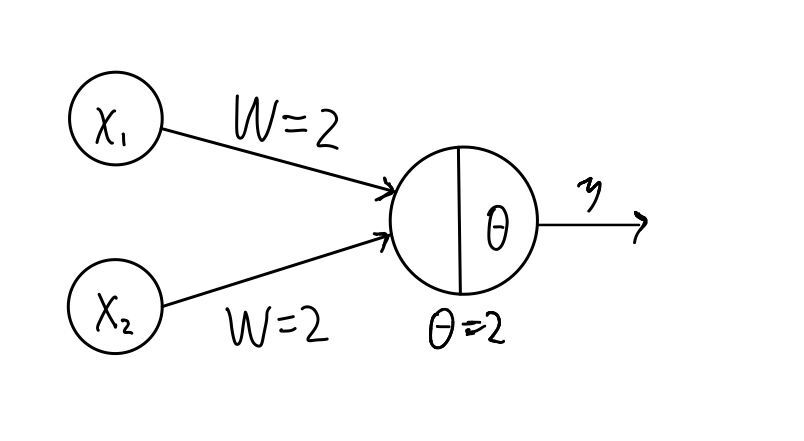
\includegraphics[width=0.3\textwidth]{or.png}
        \caption{OR}
        \label{or}
        \end{figure}
  \item NOT的感知器神经元为图\ref{not},其数学表达式为$y=f(-2x+1)$。
      \begin{figure}[h]
  	     \centering
  	     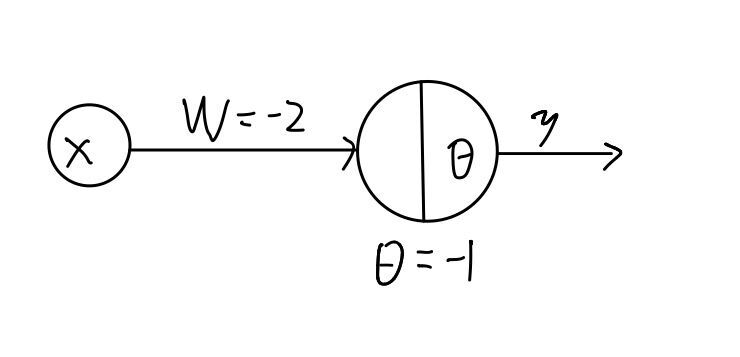
\includegraphics[width=0.3\textwidth]{not.png}
     	 \caption{NOT}
     	 \label{not}
      \end{figure}
  \item XOR的感知器神经元为图\ref{xor},因为$$x_1 \oplus {x_2}=\neg( ( \neg{x_1} \cup {x_2}) \cap (x_1 \cup \neg{x_2}))$$其中第三层神经元其实就是AND神经元。
  \begin{figure}[h]
  	\centering
  	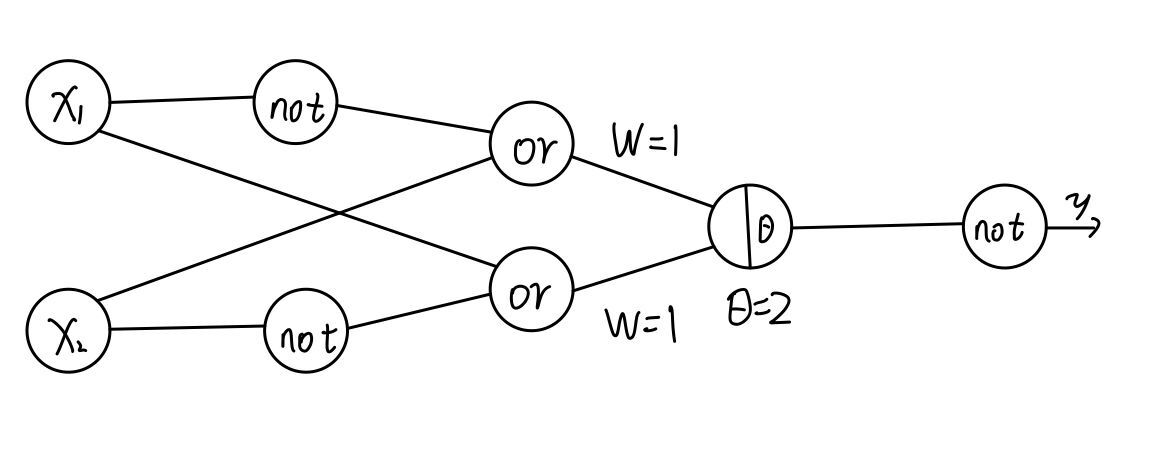
\includegraphics[width=0.5\textwidth]{xor.png}
  	\caption{XOR}
  	\label{xor}
  \end{figure}
\end{enumerate}
\end{solution}

\section*{Problem 2}
利用最小二乘法求解下列x,y关系的线性回归方程,并用单神经元表示,需要指明各参数和函数类型。
\begin{table}[!htbp]
	\centering
\begin{tabular}{|c|c|c|c|c|c|c|c|c|c|c|}% 通过添加 | 来表示是否需要绘制竖线
	\hline  % 在表格最上方绘制横线
	x&24&15&23&19&16&11&20&16&17&13\\
	\hline  %在第一行和第二行之间绘制横线
	y&92&79&97&89&64&47&83&68&71&59\\
	\hline % 在表格最下方绘制横线
\end{tabular}
\end{table}
\begin{solution}.
	\begin{enumerate}[$\bullet$]
		\item 分别令$w,b$表示权重和偏置,此线性回归问题可以表示为 $$\mathop{\arg\min}\limits_{w,b} \frac{1}{10}\sum_{i=1}^{10}(wx_i+b-y_i)^2$$
		对$w$和$b$求偏导为$0$得到$$w=3.5324,\quad b=13.4365$$。其神经元表示为图\ref{lr},其中函数$\sum$表示求和,函数$f(x)=x$。
		\begin{figure}[h]
			\centering
			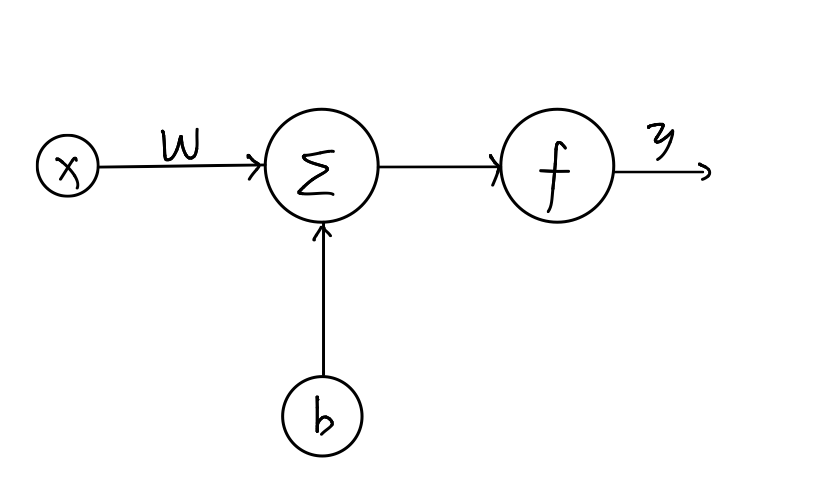
\includegraphics[width=0.3\textwidth]{lr.png}
			\caption{LR}
			\label{lr}
		\end{figure}
	\end{enumerate}
\end{solution}
\end{document}